\documentclass{amsart}

\newtheorem{theorem}{Theorem}[section]
\newtheorem{lemma}[theorem]{Lemma}

\theoremstyle{definition}
\newtheorem{definition}[theorem]{Definition}
\newtheorem{example}[theorem]{Example}
\newtheorem{xca}[theorem]{Exercise}

\theoremstyle{remark}
\newtheorem{remark}[theorem]{Remark}

\numberwithin{equation}{section}

% Some packages
\usepackage{listings, color, keyval}

% Some commands
\newcommand{\RR}{\mathbb{R}}
\newcommand{\NN}{\mathbb{N}}
\newcommand{\CC}{\mathbb{C}}
\newcommand{\II}{\mathbb{I}}
\newcommand{\KK}{\mathbb{K}}


%%% Florian

\newcommand{\Id}{\mathrm{Id}}
\renewcommand{\vec}{\textbf}
\usepackage{graphicx}
\usepackage[left=2cm,right=2cm,top=2.6cm,bottom=1.4cm,includefoot]{geometry}
\usepackage{hyperref}
\newcommand{\norm}[1]{\left\lVert#1\right\rVert}


\begin{document}

\title{Iterative Methods}

%author information
\author{Thanh-Van Huynh, Michael Thiele, Florian Wolf}
\email{thanh-van.huynh@uni-konstanz.de, michael.thiele@uni-konstanz.de, florian.2.wolf@uni-konstanz.de}

%\dedicatory{Thanks Gabriele and Christian for your great work.}

\begin{abstract}
This is a report about the findings of Thanh-Van Huynh, Michael Thiele and Florian Wolf in the exercises accompanying Iterative Methods for Linear Systems. The lecture was held by Jun.-Prof. Dr. Gabriele Ciaramella with the assistance of Christian J\"ackle in the winter term 2020/21 at the University of Constance.
\end{abstract}

\maketitle

\tableofcontents


%% ====================================================================

\section{Introduction}
In the exercises we studied optimal control problems governed by the Laplace equation. We want to solve
\begin{align}
\min\limits_{y,u\in L^2(\Omega)} J(y,u) &:= \frac{1}{2}\ \norm{y-y_d}
_{L^2(\Omega)}^2 + \frac{\nu}{2}\ \norm{u}_{L^2(\Omega)}^2\\
\text{s.t. } -\Delta y &= f+ u \text{ in } \Omega\\
y &= 0 \text{ on } \partial\Omega
\end{align}
for a regularization parameter $\nu > 0$. We are looking for a control function $u$. With discretized norm
\begin{equation*}
\norm{\vec{x}}_{L_h^2(\Omega)}^2 := h^2 \sum\limits_{j=1}^n \vec{x}_j^2
\end{equation*}
for $h>0$ small enough, such that
\begin{equation*}
A\vec{y}=\vec{f}+\vec{u}
\end{equation*}
is satisfied. Notice that we do not have any boundary conditions. One possible way of finding a solution is the so-called reduced approach: We consider $\vec{y}$ as a function of $\vec{u}$, therefore obtaining the problem
\begin{equation*}
\min\limits_{\vec{u}\in\Omega} \hat{J}(\vec{u}) := J(\vec{y}(\vec{u}),\vec{u}).
\end{equation*}


%% ====================================================================
%% ====================================================================
%% ====================================================================

%% ====================================================================

\section{Stationary Methods}
\subsection{Deriving the Optimality System}
We see that
\begin{equation*}
\norm{\vec{x}}_{L_h^2(\Omega)}^2 = h^2\ \norm{\vec{x}}_2^2
\end{equation*}
holds for arbitrary $x$. In combination with $\vec{y}=A^{-1}\left(\vec{f}+\vec{u}\right)$, we obtain
\begin{flalign*}
\min\limits_{\vec{u}\in\Omega} \hat{J}(\vec{u}) 
&=\ \frac{1}{2}\ h^2 \norm{A^{-1}\left(\vec{f}+\vec{u}\right)-\vec{y}_d}_2^2\ + \frac{\nu}{2}\ h^2 \norm{\vec{u}}_2^2\\
& =\ \frac{1}{2}\ h^2 \langle A^{-1}\left(\vec{f}+\vec{u}\right)-\vec{y}_d,A^{-1}\left(\vec{f}+\vec{u}\right)-\vec{y}_d\rangle + \frac{\nu}{2}\ h^2 \langle\vec{u},\vec{u}\rangle\\
& =\ \frac{1}{2}\ h^2  \left(A^{-1}\left(\vec{f}+\vec{u}\right)-\vec{y}_d\right)^{\top} \left(A^{-1}\left(\vec{f}+\vec{u}\right)-\vec{y}_d\right) + \frac{\nu}{2}\ h^2 \vec{u}^{\top}\vec{u}.
\end{flalign*}
As we know that a solution $\vec{u}$ to the problem above has to satisfy $\nabla\hat{J}(\vec{u})=0$, this results in
\begin{equation*}
\nabla \hat{J}(\vec{u}) = h^2 A^{-1} \left(A^{-1} (\vec{f}+\vec{u})-\vec{y}_d\right) + \nu h^2\vec{u} = 0.
\end{equation*}
We can do the following transformations
\begin{flalign*}
h^2 A^{-1} \left(A^{-1} (\vec{f}+\vec{u})-\vec{y}_d\right) + \nu h^2\vec{u} &= 0\\
A^{-1} \left(A^{-1} (\vec{f}+\vec{u})-\vec{y}_d\right) + \nu \vec{u} &=0\\
A^{-1} A^{-1} (\vec{f}+\vec{u})-A^{-1}\vec{y}_d + \nu \vec{u} &=0\\
A^{-1} A^{-1} \vec{f}+A^{-1} A^{-1}\vec{u}-A^{-1}\vec{y}_d + \nu \vec{u} &=0\\
A^{-1} A^{-1} \vec{u} + \nu \vec{u} &=A^{-1}\vec{y}_d-A^{-1} A^{-1}\vec{f}\\
\left(\nu\text{I}+A^{-1} A^{-1}\right) \vec{u} &=A^{-1}\left(\vec{y}_d-A^{-1}\vec{f}\right)
\end{flalign*}
and derive the optimality system
\begin{equation}
\left(\nu\text{I}+A^{-2}\right) \vec{u} =A^{-1}\left(\vec{y}_d-A^{-1}\vec{f}\right) \label{eq:normalOptimalitySystem}
\end{equation}
or alternatively
\begin{equation}
\left(A^2\nu+\text{I}\right) \vec{u} =A\vec{y}_d-\vec{f}. \label{eq:factoredOptimalitySystem}
\end{equation}


%% ====================================================================



\subsection{Laplace Matrices}
First, we implement a function \texttt{FD\_Laplacian} to create the Finite Difference matrix representation of the Laplace operator in sparse.
Depending on whether we choose $d=1$ or $d=2$, we obtain the 1D Laplace Matrix 
$$ T_1 = 
\begin{pmatrix}
-2 & 1 & & & \\
1 & -2 & 1 & & \\
& \ddots & \ddots & \ddots & \\
%& & \ddots & \ddots & 1 \\
%& & & 1 & -2  
\end{pmatrix} \in\RR^{m\times m}
$$
or the 2D Laplace Matrix (by using the Kronecker product $\otimes$)
$$ T_2 = \text{I}_m \otimes T_1 + T_1 \otimes \text{I}_m= 
\begin{pmatrix}
T_1 & \text{I}_m & & \\
\text{I}_m & T_1 & \text{I}_m & \\
& \ddots & \ddots & \ddots
\end{pmatrix} \in\RR^{m^2\times m^2}.
$$

\begin{lstlisting}[mathescape, language=Pascal, title=FD\_Laplacian,
frame=single, numbers=left, numberstyle=\tiny, tabsize=2,
morekeywords={Enter, Return, elif}, deletekeywords={of,or}, keywordstyle=\bfseries]{}
Enter: matrix dimension $m\in\NN$, $d=\{1,2\}$ choosing 1D or 2D
Return: Laplace matrix $T\in\RR^{m\times m}$
diag = -2*sparse.identity($m$)
onesUpper = sparse.eye($m,k=1$)
onesLower = sparse.eye($m,k=-1$)
$T$ = diag + onesUpper + onesLower
if $d==2$:
	eye = sparse.eye($m$)
	$T$ = sparse.kron(eye,$T$) + sparse.kron($T$,eye)
return($T$)
\end{lstlisting}

%% ====================================================================

\subsection{Fast Poisson Solver}
Now, we implement the Fast Poisson Solver \texttt{Fast\_Poisson} to efficiently solve a linear system $Au=b$. As we do not have any boundary conditions, we have a simpler implementation:

\begin{lstlisting}[mathescape, language=Pascal, title=Fast\_Poisson,
frame=single, numbers=left, numberstyle=\tiny, tabsize=2,
morekeywords={Enter, Return, elif}, deletekeywords={of}, keywordstyle=\bfseries]{}
Enter: matrix $V$ of eigenvectors of the matrix $A\in\RR^{m\times m}$, 
vector $\lambda$ of eigenvalues of the matrix $A$, 
right-hand side $b$ of the linear system
Return: solution $u$ of the linear system $Au=b$
$B$ = reshape($b,(m,m)$)
$\tilde{B} = (V^{\top}(V^{\top}B)^{\top})^{\top}$
for i in 0:m
	for j in 0:m
			$\tilde{u}_{ij}=(\tilde{B}_{i,j})/(\lambda_i+\lambda_j)$
$U = (V(V\tilde{U})^{\top})^{\top}$
$u$ = reshape($U,m^2$)
return($u$)
\end{lstlisting}

%% ====================================================================

\subsection{Convergence Analysis}
Now, we solve the system (\ref{eq:normalOptimalitySystem}) by the stationary iteration
\begin{equation}
\vec{u}^{n+1} = -\frac{1}{\nu} A^{-2}\vec{u}^n + \frac{1}{\nu} A^{-1} (\vec{y}_d-A^{-1}\vec{f})
\end{equation}
and analyze its convergence behavior for different $m$ and $\nu$.
\subsubsection{Eigenvectors and eigenvalues of the laplace matrices}
As we have seen in the section regarding the stationary solver and we will see this again, if we consider solving \eqref{eq:normalOptimalitySystem} 
using the conjugated gradient method, the poisson solver is the key, to get a fast solution to the $A^{-1}$ problem. The solver requires a decomposition
of the matrix $V$ in diagonalized form. In the beginning we achieved this task using \texttt{scipy.sparse.eigs}. Luckily the eigenvectors and eigenvalues
of the one dimensional laplace matrix are easy to calculate by hand, exploiting its Toeplitz-structure. For the $m\times m$ one-dimensional laplace, we 
get the following eigenvalues
\begin{align*}
\lambda_k = -2 + 2 \cos \left( \frac{\pi k}{n+1} \right), \quad k=1,\ldots, m
\end{align*} 
and the corresponding eigenvectors with entries
\begin{align*}
(\vec{v}_k)_i = \sin\left(\frac{i\cdot \pi k}{m+1} \right), \quad i,k=1,\ldots,m
\end{align*}
Now we can include these manually to get a more exact and especially quicker solver.

To get the eigenvectors and eigenvalues of the two-dimensional laplace matrix, we use problem 10 of REFERENCE TO THE BOOK and proof its third bullet 
point. Therefore we use the formula $(A \otimes B)(C \otimes D) = (AC) \otimes (BD)$. For $j,k \in \{1, \ldots, m\}$ arbitrary we get for $\lambda := 
\lambda_j + \lambda_k$ and $\vec{v} := \vec{v}_j \otimes \vec{v}_k$ that
\begin{align*}
A\vec{v} &= \left(\text{I}_m \otimes T_1 + T_1 \otimes \text{I}_m \right) \vec{v}\\
&= \left( \text{I}_m \otimes T_1\right)\left(\vec{v}_j \otimes \vec{v}_k\right) + \left( T_1 \otimes \text{I}_m\right)\left(\vec{v}_j \otimes \vec{v}_k\right)\\
&= \left( \vec{v}_j \otimes \lambda_k \vec{v}_k\right) + \left( \lambda_j\vec{v}_j \otimes  \vec{v}_k\right)\\
&= \lambda_k\left( \vec{v}_j \otimes  \vec{v}_k\right) + \lambda_j\left( \vec{v}_j \otimes  \vec{v}_k\right)\\
&= \lambda \vec{v}
\end{align*}
Therefore the eigenvectors and eigenvalues of the two-dimensional laplace are obtained by using the kronecker product of the one-dimensional eigenvectors
and summing up the one-dimensional eigenvalues. We will use the eigenvalues, to calculate the condition number of the matrix in the section
about Krylov methods.
%% ====================================================================

\subsection{Damped Jacobi}

%% ====================================================================
\newpage
\section{Krylov Methods}
%% ====================================================================

\subsection{Convergence Analysis}
In this part of the project we want to use the fact, that the matrix arising in our disretization is symmetric and positive definite. For this reason we 
want to apply the conjugated gradient (CG) method, to solve our systems \eqref{eq:normalOptimalitySystem} and \eqref{eq:factoredOptimalitySystem}.
For the first system we use the already implemented fast poisson solver, to get a matrix free version of the left-hand side. In the second case we 
construct our sparse matrices and use the \texttt{scipy.sparse.linalg.LinearOperator} method, to create a linear operator of our left-hand side of the 
equation. So in both cases the solution process is completely matrix-free.


Looking at figure \ref{fig:CG-convergence}, we can see the  convergence behaviour for the two systems. In the plots $\nu$ ist getting bigger going from top to bottom and $m$ is getting bigger going from left to right.
\begin{figure}[h!]
\centering
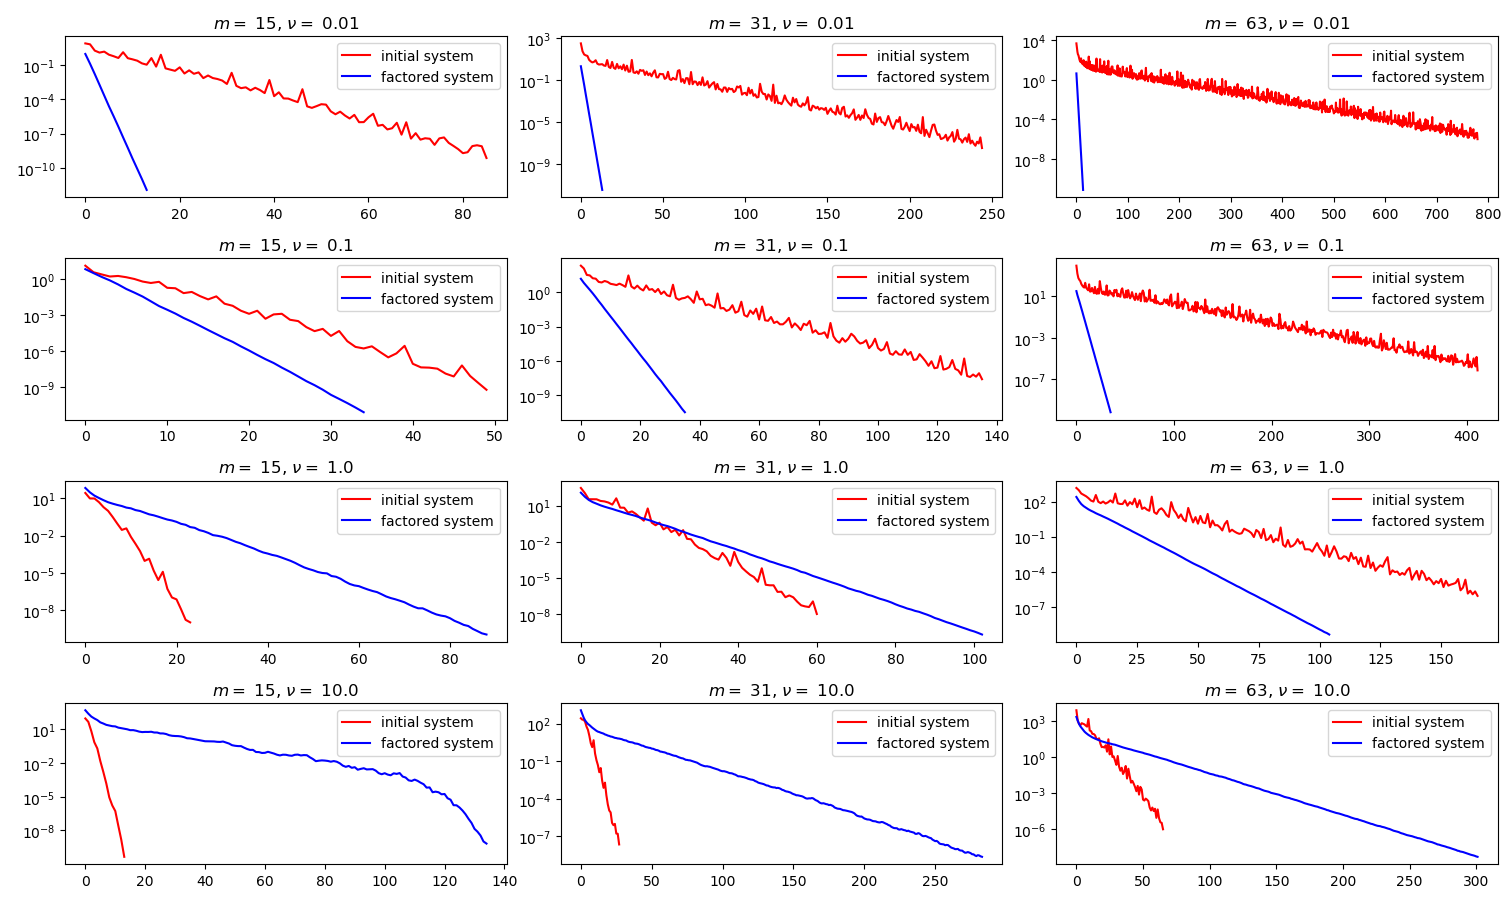
\includegraphics[scale=0.56]{./imgs/CG_analysis}
\caption{Convergence behaviour for different values of $m$ and $\nu$ using CG to solve the systems. The x-axis is representing the number of iterations
and the y-axis the 2-norm of the residuals.}
\label{fig:CG-convergence}
\end{figure}
As you can directly see in the plots, the solution process of both systems is getting worse, as the size of the matrix increases. Meanwhile, the behaviour 
regarding different values of $\nu$ is more interesting. While the convergence of the initial optimality systems solution is getting slower and slower if 
$\nu$ increases, the convergence rate of the factored system is getting faster and faster. So the systems behave in an opposite way, regarding the size of 
$\nu$.

%% ====================================================================
\subsection{Conditional Number}
One can explain this, if we take a closer look at the conditon number of the systems for the upper combinations of $\nu$ and $m$. We can see this in 
figure \ref{fig:CG-conditionNumber}.
\begin{figure}[h!]
\centering
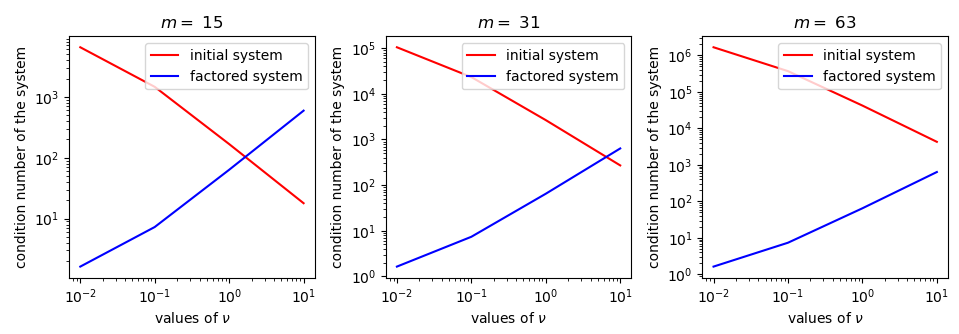
\includegraphics[scale=0.65]{./imgs/CG_conditionNumber}
\caption{Condition numbers of both systems for different values of $m$ and $\nu$ represented in a double-logarithmic plot.}
\label{fig:CG-conditionNumber}
\end{figure}
The three plots of the condition number explain really good, why we get the upper type of convergence behaviour. While both condition numbers get overall
bigger from left to right (so with increasing matrix size due to bigger $m$), one can clearly see in each of the plots that the systems have opposed 
curves.

While the factored system \eqref{eq:factoredOptimalitySystem} is worse conditioned for bigger $\nu$, the condition number of the initial system 
gets better the bigger $\nu$ is. Looking at the formulas \eqref{eq:normalOptimalitySystem} and \eqref{eq:factoredOptimalitySystem} this should now be 
really obvious.
In \eqref{eq:factoredOptimalitySystem} we factor our matrix $A^2$ by $\nu$, so the bigger $\nu$ is, the worse the condition number gets. In the initial 
system \eqref{eq:normalOptimalitySystem} the identity matrix with factor $\nu$ dominates the diagonal of the left-hand side for bigger $\nu$. So the 
condition number is getting better and better as $\nu$ increases.

%% ====================================================================

\section{Multigrid}

%% ====================================================================

In our last section we use multigrid methods to solve our problems \eqref{eq:normalOptimalitySystem} and \ref{eq:factoredOptimalitySystem}. These problems can be derived by discretization, as shown in the introduction. So we are able to apply multigrid methods. We have already seen two stationary methods:
\begin{equation}
\vec{u}^{n+1}    = - \frac{1}{\nu} A^{-2} \vec{u}^n+ \vec{f}
\label{eq: stationaryMethod}
\end{equation}
and 
\begin{equation}
\vec{u}^{n+1}    =  \vec{u}^n+ \omega D^{-1}  (\vec{f} - (\nu \Id + A^2) \vec{u}^n)
\label{eq: dampedJacobi}
\end{equation}
In the following we will refer to \eqref{eq: stationaryMethod} as the stationary method, in order to distinguish this method from \eqref{eq: dampedJacobi} which is called damped Jacobi method with damping parameter $\omega \in (0,1] $. We used \eqref{eq: stationaryMethod} to solve  \eqref{eq:normalOptimalitySystem} and \eqref{eq: dampedJacobi} to solve \eqref{eq:factoredOptimalitySystem}. Now we want to apply \eqref{eq: stationaryMethod} and \eqref{eq: dampedJacobi} as smoother in a multigrid methods. In both multigrid methods we use the interpolation matrix $P$ and the full weighting restriction matrix $R:= \frac{1}{2} P^T$  in our coarse correction step. Furthermore we do 2 Pre-Smoothing and 2 Post-Smoothing steps. 
\subsection{Stationary Method as Smoother}
First we analyse \eqref{eq: stationaryMethod} and it's corresponding multigrid method. We expect that the convergence of our multigrid methods gets better for rising $\nu$. Because regarding the notation of the script $M^{-1} N = - \frac{1}{\nu} A^{-2} $ is the iteration matrix of the stationary method. Therefore our stationary method converges faster for $\nu $ rising, which is shown in \ref{sec:DampedJacobi}. For smaller $\nu$ we can expect slower or not even convergence at all, if the stationary method does not converge. 


\begin{figure}[h!]
	\centering
	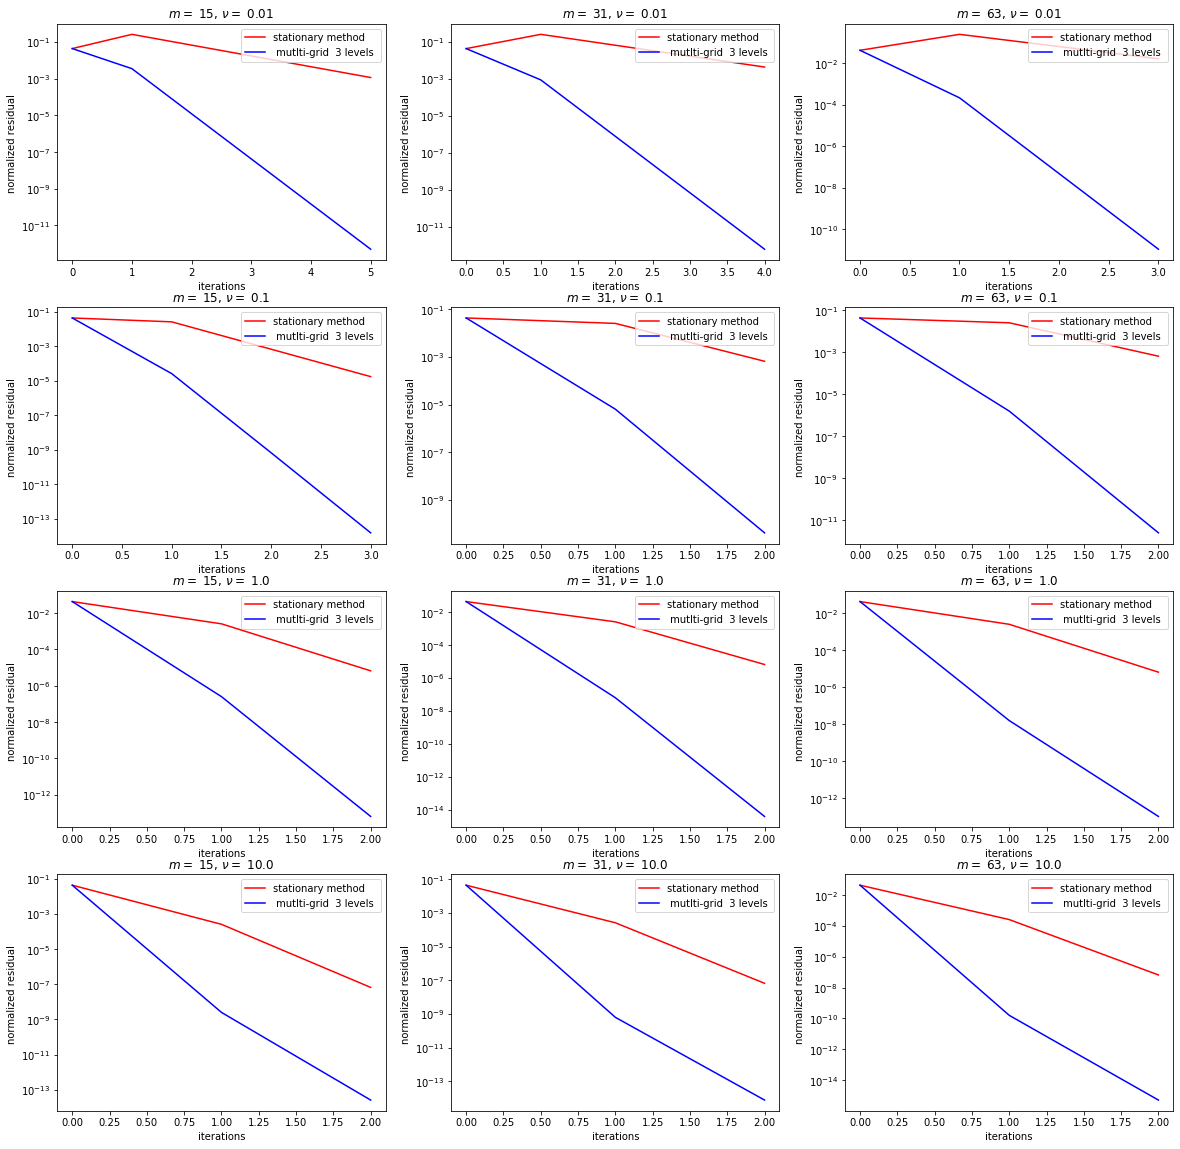
\includegraphics[scale=0.4]{./imgs/multigrid_stat_comparison_tiny}
	\caption{Number of iterations of multigrid in comparison with the stationary method for different $\nu$ and $m$}
	\label{fig: multigridStationary}
\end{figure}
Now let us check, if our predictions were right. From figure \ref{fig: multigridStationary} we can observe, that our multigrid method converges only for huge $\nu $. This can be explained by the fact, that our sationary method converges only for huge $\nu$. In this case the term $\nu \Id$ dominates $\nu \Id + A^{-2}$ and we get a iteration which would be similar to a jacobi one. As bigger $m$ gets, $\nu$ needs to grow faster to achieve this effect. Therefore our multigrid method is not independent of the size $m$, because our stationary method can stop converging for $m$ rising. Though provided that our multigrid method converges, it needs only a few iterations. In this case our method is extremly quick  


%% ====================================================================

\subsection{Damped Jacobi as Smoother}
<<<<<<< HEAD
\hfill
=======
Now we want to analyse the multigrid method with damped jacobi as smoother. We set $\omega= 0.5$, so we go half the way of every step. Let's make some predictions what happens, if we run our multigrid method. First we expect, that the multigrid method will be faster for shrinking $\nu$ and slower for bigger $\nu$. Because of $I + \nu A^2$ is diagonal dominant for small $\nu$, and Jacobi converges for such systems. For rising $\nu$, we'll lose this effect. Nevertheless, $A^2$ is block tridiagonal:
\begin{align*}
A^2\\
= (I \otimes T + T \otimes I)^2 \\
= 2  \cdot T \otimes T + T^2 \otimes \Id + \Id \otimes T^2 
\end{align*}
That's why Jacobi should still produces reasonable results. 
\begin{figure}[h!]
	\centering
	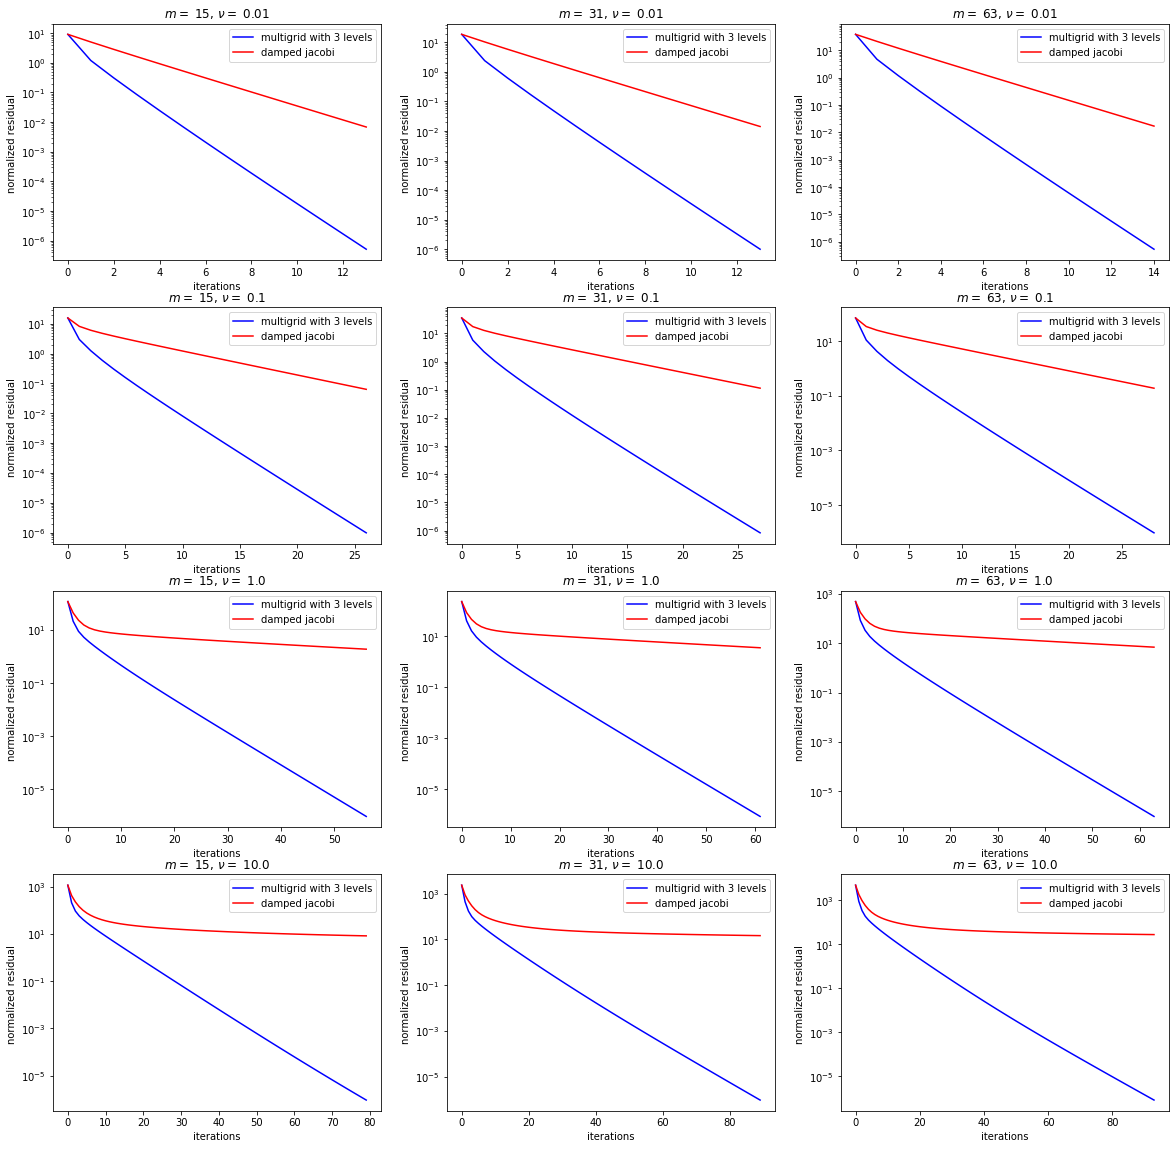
\includegraphics[scale=0.4]{./imgs/multigrid_jac_comparison_tiny}
	\caption{Number of iterations of multigrid in comparison with damped jacobi for different $\nu$ and $m$}
	\label{fig: multigridJacobi}
\end{figure}

Again let's verify our predictions. In figure \ref{fig: multigridJacobi} we can see exactly, what we expected. Our method is great for solving problems with small $\nu$. Though for very small $\nu$ we come close to:
\[
\Id   \vec{v} = \vec{f}
\] 
and the solution isn't so meaningful.
Moreover we can see, that the multigrid method converges slower for $\nu$ rising. So thats again, what we predicted. From figure \ref*{fig: multigridJacobi} we really see, that our multigrid method is independent of the size $m$. We are able to observe this phenomenon in nearly every row. 
>>>>>>> 05b9222477d001209b1681ef506f820b6c8e50a1
\end{document}
